\section{Diagnostic Analysis}
\label{sec:diagnostic}

While global metrics provide a high-level overview of model performance, they often obscure critical, localized failure modes~\cite{}. To uncover these systemic vulnerabilities, we perform an exhaustive error analysis across categorical, spatial, depth, and scale dimensions.

\subsection{Semantic and Spatial Vulnerabilities}

\textbf{Boundary Degradation:} Despite competitive overall mIoU scores, both CNN and ViT architectures exhibit profound failures near semantic contours. Anomalies located near boundaries of weak-performing classes (such as Pole, Rider, Fence, Motorcycle, and Wall) are frequently absorbed into background noise. We observe a massive surge in the False Positive Rate (FPR95) when transitioning from flat central regions to boundary areas (e.g., FPR95 increasing from approximately 60\% to over 90\%). Architecturally, CNNs struggle here due to fixed receptive fields that blur edges, while ViTs suffer from coarse patch tokenization ($16 \times 16$) that inherently degrades high-frequency spatial boundaries.

% --- INIZIO CODICE IMMAGINE 1 ---
\begin{figure}[htbp]
  \centering
  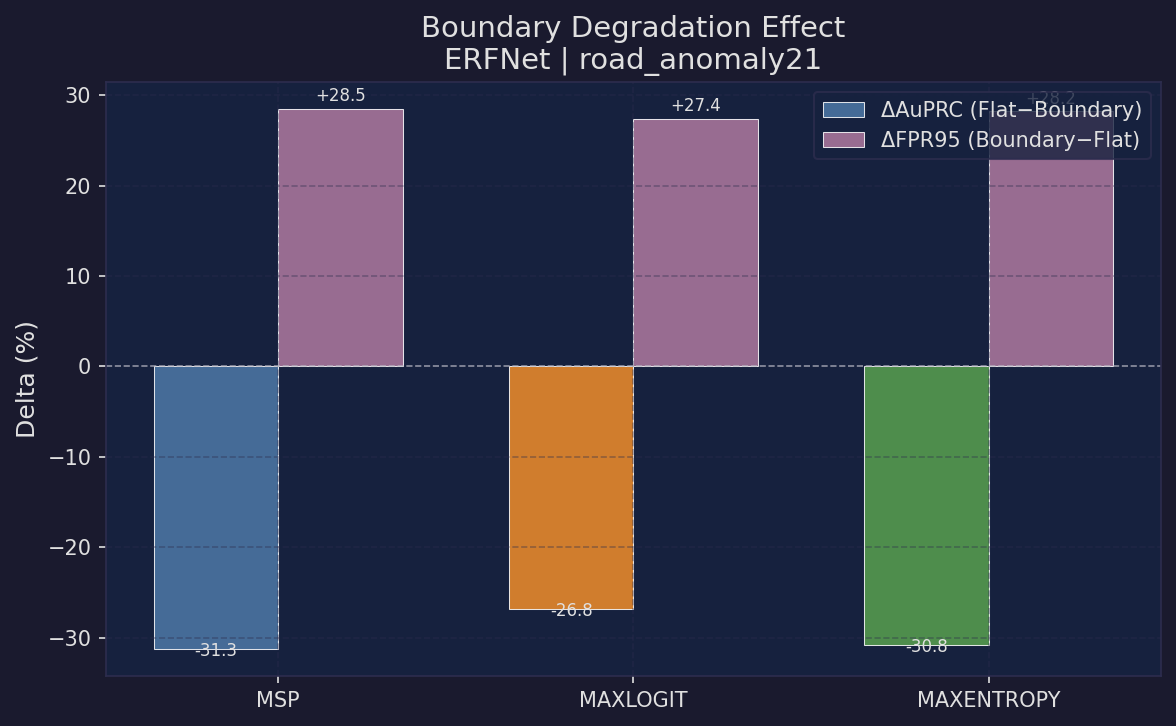
\includegraphics[width=\linewidth]{analysis_reports/boundary_delta_road_anomaly21_ERFNet.png}
  \caption{Boundary Uncertainty in ERFNet. The False Positive Rate (FPR95) dramatically increases at semantic boundaries compared to flat regions, creating critical blind spots for anomaly detection.}
  \label{fig:boundary_uncertainty}
\end{figure}
% --- FINE CODICE IMMAGINE 1 ---

\textbf{Depth-Dependent Vertical Blindness:} Evaluating performance across horizontal depth bands reveals a catastrophic collapse in Out-of-Distribution (OoD) detection for distant objects. In the furthest depth band, both models are virtually blind to anomalies, with AuPRC dropping to critically low levels (e.g., $<10\%$). Models only react reliably when obstacles enter the immediate mid-to-near vicinity. This "Vertical Blindness" indicates that generic optimization fails to learn scale-distance invariance for anomalies.

% --- INIZIO CODICE IMMAGINE 2 ---
\begin{figure}[htbp]
  \centering
  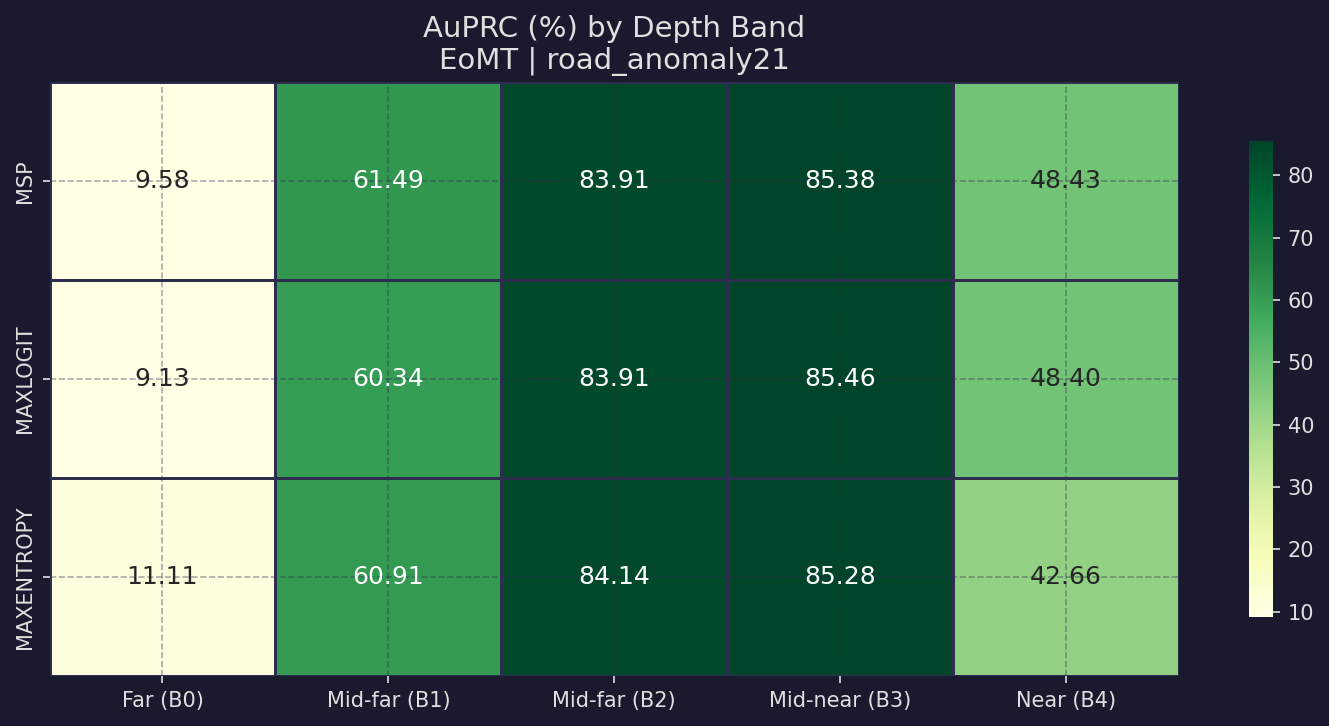
\includegraphics[width=\linewidth]{analysis_reports/depth_heatmap_auprc_road_anomaly21_EoMT.png}
  \caption{Depth-dependent Vertical Blindness. Heatmap analysis on RoadAnomaly21 reveals that EoMT detection performance collapses for objects in the far distance, reacting only when anomalies are in the immediate vicinity.}
  \label{fig:depth_blindness}
\end{figure}
% --- FINE CODICE IMMAGINE 2 ---

\subsection{Object Typology: The Scale Paradox vs. The Scale Gap}

Isolating anomalies by pixel area uncovers diametrically opposed failure modes between the two architectures.

\textbf{The ERFNet Scale Paradox:} Counter-intuitively, the CNN's False Negative Rate (FNR) degrades catastrophically as the anomaly size increases, reaching FNRs above 90\% on massive objects. This failure stems from the limited receptive field: massive anomalies engulf the entire filter, depriving the network of contextual contrast. Forced to rely solely on local textures, the CNN blindly assigns high In-Distribution confidence to large anomalies.

\textbf{The EoMT Scale Gap:} Conversely, the ViT demonstrates excellent detection for massive obstacles but acts as a low-pass filter that suppresses small-scale debris. For objects under a thousand pixels, the AuPRC approaches zero (with FNR $>50\%$). The patch tokenization process dilutes high-frequency details of small obstacles into dominant background patches. While increasing the input resolution mitigates this Scale Gap, it severely penalizes frames-per-second (FPS) throughput, introducing an unacceptable resolution-latency trade-off for real-time applications.

% --- INIZIO CODICE IMMAGINE 3 ---
\begin{figure}[htbp]
  \centering
  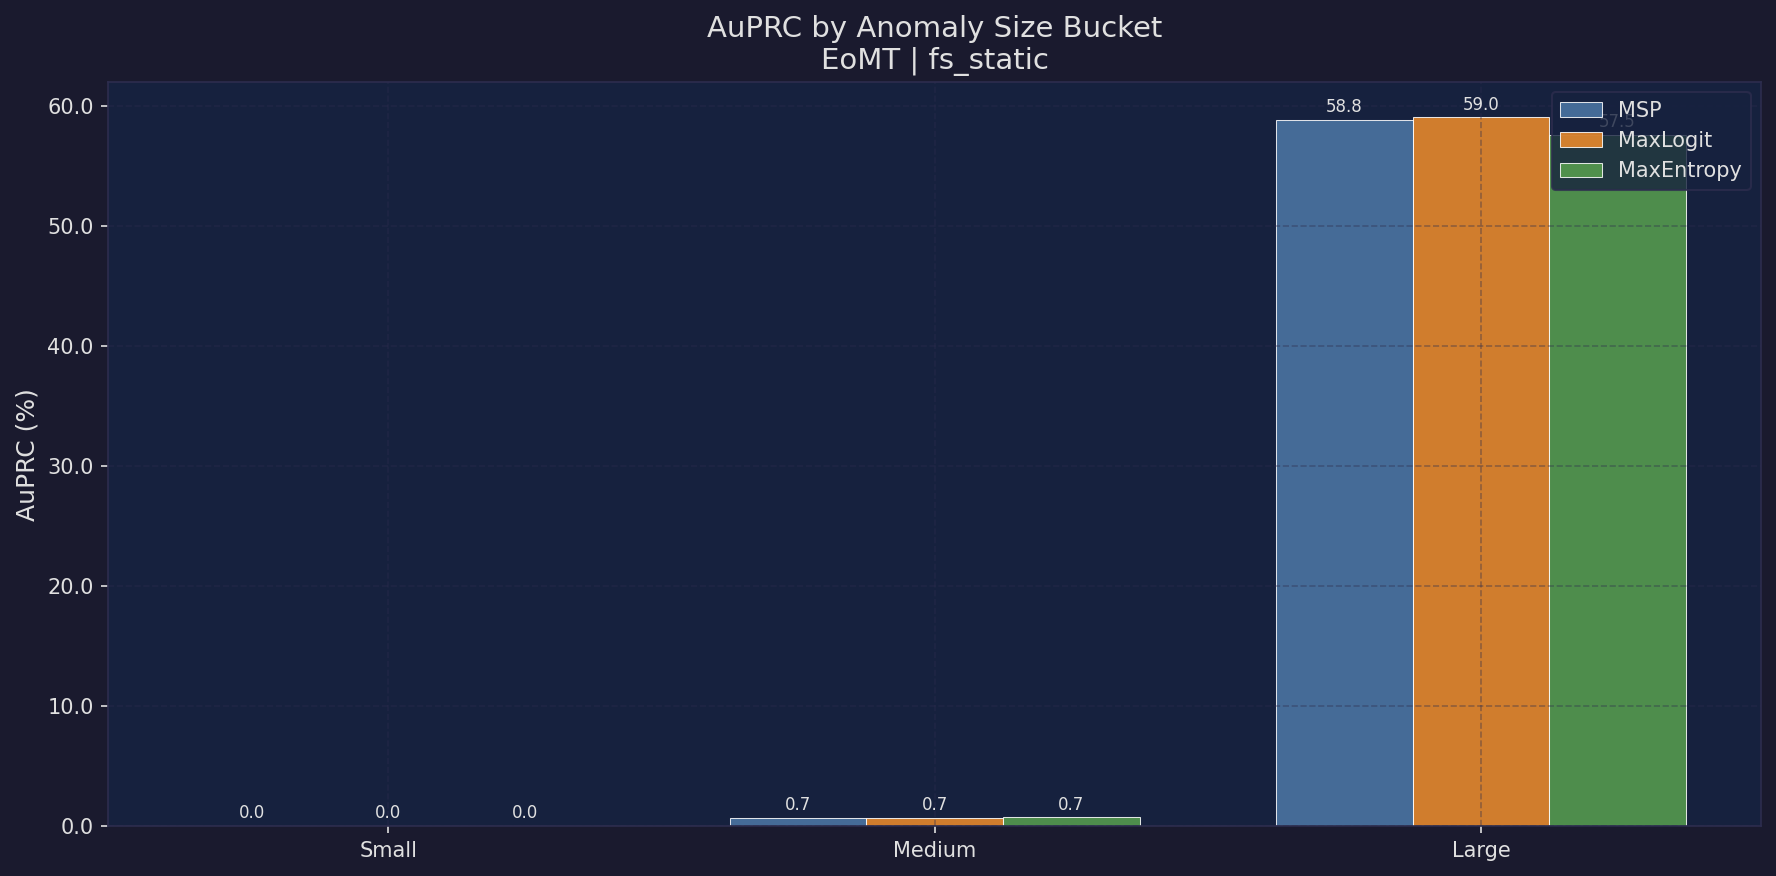
\includegraphics[width=\linewidth]{analysis_reports/size_auprc_fs_static_EoMT.png}
  \caption{The Scale Gap in Vision Transformers. Evaluating EoMT on FS Static demonstrates a binary behavior: near-zero AuPRC for small objects, contrasting with strong detection capabilities for massive obstacles.}
  \label{fig:scale_gap}
\end{figure}
% --- FINE CODICE IMMAGINE 3 ---

\subsection{Taxonomic Absorption and Attention Failure}

Our evaluation exposes a phenomenon of "Taxonomic Absorption," where models forcibly anesthetize anomalies by mapping them into familiar In-Distribution categories. For example, EoMT exhibits a strong bias, absorbing roughly half of all OoD pixels into "Road" or "Vegetation", effectively hallucinating safe drivable surfaces or background scenery over critical hazards. Similarly, ERFNet displays alarming confusion peaks towards classes like "Train" and "Car".

Inspection of the ViT's self-attention maps confirms this failure mechanism. Instead of isolating the anomalous tokens, the attention weights actively bypass small-scale anomalies, converging entirely on surrounding dominant background regions. If an object's dimensions cannot influence the global tokens, the network's uncertainty signals fail to trigger.

% --- INIZIO CODICE IMMAGINE 4 e 5 ---
\begin{figure}[htbp]
  \centering
  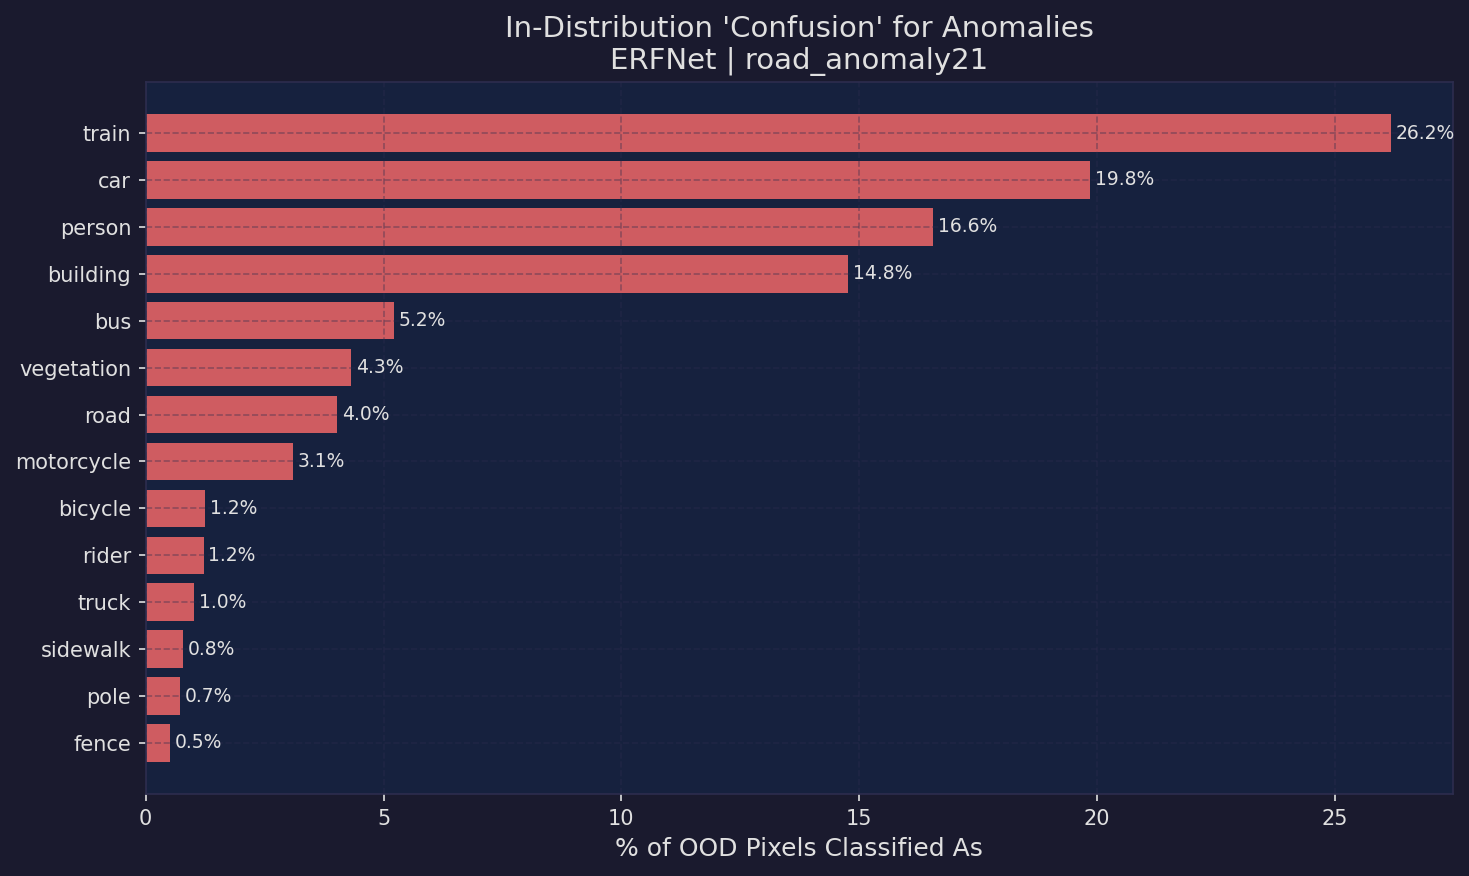
\includegraphics[width=\linewidth]{analysis_reports/confusion_bar_road_anomaly21_ERFNet.png}
  \caption{Taxonomic Absorption in ERFNet. Anomalies are frequently misclassified into familiar In-Distribution categories (e.g., Train, Car), neutralizing the Out-of-Distribution score.}
  \label{fig:taxonomic_absorption}
\end{figure}

\begin{figure}[htbp]
  \centering
  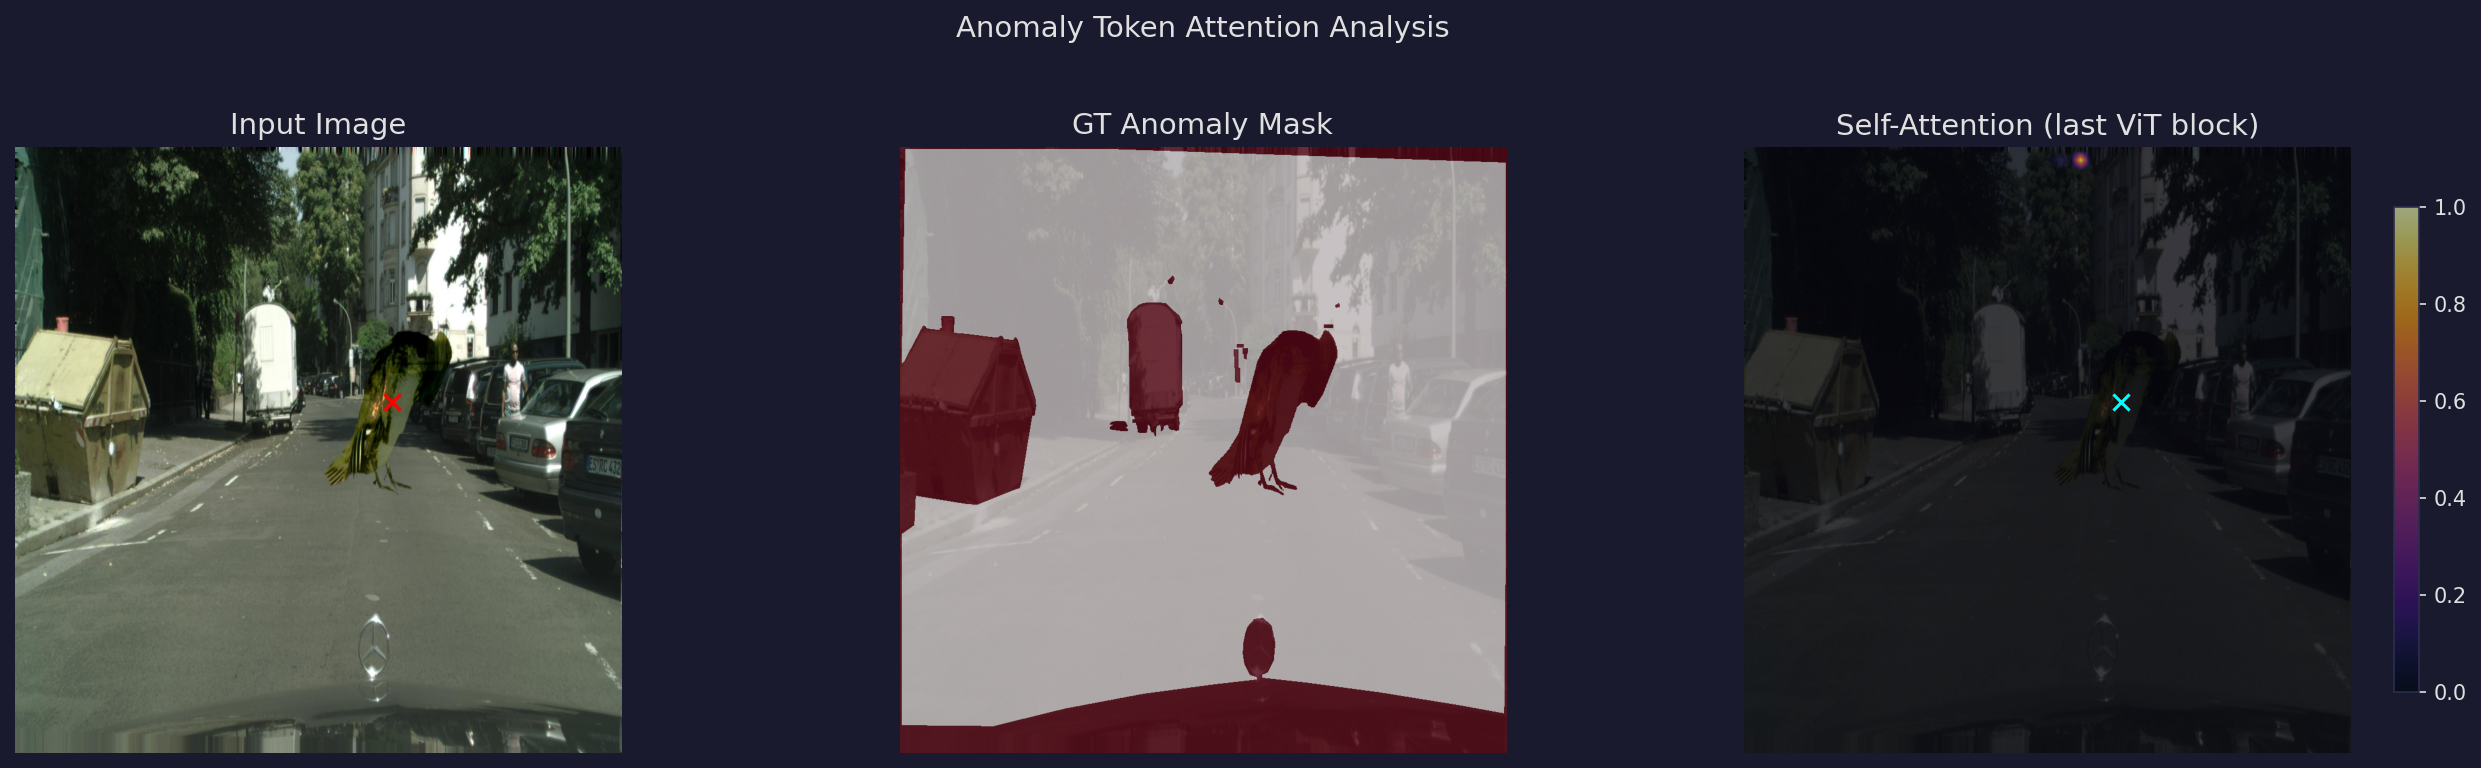
\includegraphics[width=\linewidth]{analysis_reports/attention_overlay_fs_static.png}
  \caption{Attention Map Failure in EoMT. The Vision Transformer's attention weights bypass small-scale anomalies, converging entirely on dominant background classes like Vegetation or Building.}
  \label{fig:attention_failure}
\end{figure}
% --- FINE CODICE IMMAGINE 4 e 5 ---